\section{State of the Art, Objectives, Contributions}

%\begin{frame}
%\frametitle{Template Attack}
% \begin{textblock}{5}(10,2)
% \important{$\vaLeakVec\in \mathbb{R}^D$\\
%  Curse of dimensionality!}
% \end{textblock}
%\begin{itemize}
%\item Profiling phase (using profiling traces under known $\sensRandVar$)
%\begin{itemize}
%\item \uncover<7->{manage de-synchronization problem}
%\item \uncover<6->{mandatory dimensionality reduction}
%\item \uncover<6->{Gaussian hypothesis \cite{Chari2003}}
%\item \uncover<6->{Variants: \emph{pooled} version \cite{choudary2014efficient}, linear regression \cite{schindler2005stochastic}}
%\item \uncover<2->{estimate \only<2-4>{$\prob[\vaLeakVec|\sensRandVar=\sensVar]$ (generative model)} \only<5-6>{\textcolor{blue}{$\prob[\vaLeakVec|\sensRandVar=\sensVar]$}} \only<7->{\textcolor{blue}{$\prob[\important{\varepsilon(\vaLeakVec)}|\sensRandVar=\sensVar]$}}for each value of $\sensVar$}
%\end{itemize}
%\item Attack phase ($N$ attack traces $\vLeakVec_i$, e.g. with known plaintexts $p_i$)
%
%\only<1-4>{ \begin{itemize}
%\item[] \textcolor{white}{Log-likelihood score for each key hypothesis $k$
%\begin{equation*}
%d_k = \sum_{i=1}^{N}\log \prob[\vaLeakVec=\vLeakVec_i | Z=f(p_i,k)]
%\end{equation*}
%}
%
%\item\textcolor{white}{A-posteriori probability score for each key hypothesis $k$
%\begin{align*}
%\pdf_{\given{\sensRandVar}{  \vaLeakVec = \vLeakVec}}(\sensVar) &= \frac{\pdf_{\given{\vaLeakVec}{\sensRandVar = \sensVar}}(\vLeakVec)\pdf_{\sensRandVar}(\sensVar)} {\pdf_{\vaLeakVec}(\vLeakVec)}\text{Bayes' theorem}\\
%d_{\keyVar} &= \prod_{i=1}^{\nbAttackTraces} \pdf_{\given{\sensRandVar}{\vaLeakVec = \vLeakVec_i}}(\sensFunction(\keyVar,\publicParVar_i) ) \mbox{ ,}
%\end{align*}
%}
%\end{itemize}
%}
%\only<5-6>{\begin{itemize}
%\item Log-likelihood score for each key hypothesis $k$
%\begin{equation*}
%d_k = \sum_{i=1}^{N}\log \textcolor{blue}{\prob[\vaLeakVec=\vLeakVec_i | Z=f(p_i,k)]}
%\end{equation*}
%
%\item A-posteriori probability score for each key hypothesis $k$
%\begin{align*}
%\pdf_{\given{\sensRandVar}{  \vaLeakVec = \vLeakVec}}(\sensVar) &= \frac{\pdf_{\given{\vaLeakVec}{\sensRandVar = \sensVar}}(\vLeakVec)\pdf_{\sensRandVar}(\sensVar)} {\pdf_{\vaLeakVec}(\vLeakVec)} \text{Bayes' theorem}\\
%d_{\keyVar} &= \prod_{i=1}^{\nbAttackTraces} \pdf_{\given{\sensRandVar}{\vaLeakVec = \vLeakVec_i}}(\sensFunction(\keyVar,\publicParVar_i) ) \mbox{ ,}
%\end{align*}
%\end{itemize}
%}
%\only<7->{\begin{itemize}
%\item Log-likelihood score for each key hypothesis $k$
%\begin{equation*}
%d_k = \sum_{i=1}^{N}\log \textcolor{blue}{\prob[\important{\varepsilon(
%\vaLeakVec)}=\important{\varepsilon(
%\vLeakVec_i)} | Z=f(p_i,k)]}
%\end{equation*}
%
%
%\item A-posteriori probability score for each key hypothesis $k$
%\begin{align*}
%\pdf_{\given{\sensRandVar}{  \vaLeakVec = \vLeakVec}}(\sensVar) &= \frac{\pdf_{\given{\vaLeakVec}{\sensRandVar = \sensVar}}(\vLeakVec)\pdf_{\sensRandVar}(\sensVar)} {\pdf_{\vaLeakVec}(\vLeakVec)} \text{Bayes' theorem}\\
%d_{\keyVar} &= \prod_{i=1}^{\nbAttackTraces} \pdf_{\given{\sensRandVar}{\vaLeakVec = \vLeakVec_i}}(\sensFunction(\keyVar,\publicParVar_i) ) \mbox{ ,}
%\end{align*}
%\end{itemize}
%}
%
%\end{itemize}
%
%
%\end{frame}

\begin{frame}
\frametitle{Notations}
\begin{block}{Notations and generalities}
\begin{itemize}
\item Side-channel traces: realizations of a random vector $\vaLeakVec \in \mathbb{R}^D$  
\item $D$ is the number of time samples (or features)
\item Target: a \emph{sensitive} variable $Z = f(\mathrm{e,k})$ in $\sensVarSet = \{\sensVarValue{1}, \dots, \sensVarValue{|\sensVarSet|}\}$
%\item each label $\sensVarValue{i}$ identifies a \emph{class}
\end{itemize}
\end{block}
\vspace{-5pt}
\begin{block}{Profiling attack scenario}
\begin{itemize}
\item labelled traces $\setDataTrain = (\vLeakVec_i, e_i, k_i)_{i=1}^N$, acquired under known secrets
\item attack traces $\setDataAttack = (\vLeakVec_i, e_i)_{i=1}^{N_a}$ acquired under unknown secrets
\end{itemize}
\end{block}
\end{frame}




\begin{frame}
\frametitle{Profiling Attack}
\only<4->{
 \begin{textblock}{5}(10,2)
 \important{$\vaLeakVec\in \mathbb{R}^D$\\
  Curse of dimensionality!}
 \end{textblock}
}

\textbf{Profiling phase}
\begin{itemize}
\uncover<7->{\item \textcolor{blue}{manage de-synchronization problem [$\setDataTrain \longrightarrow \rho\colon \mathbb{R}^D\rightarrow\mathbb{R}^D$]}}
\uncover<6->{\item \textcolor{red}{mandatory dimensionality reduction [$\setDataTrain \longrightarrow \extract\colon\mathbb{R}^D\rightarrow \mathbb{R}^C$]}}
\item estimate
\begin{itemize}
\item $\pdf_{\given{\only<1-5>{\vaLeakVec}\only<6>{\textcolor{red}{\extract}{(\vaLeakVec)}}\only<7>{\textcolor{red}{\extract}{(\textcolor{blue}{\rho}(\vaLeakVec)})}}{\sensRandVar = \sensVar}}$\uncover<2->{\ $\pdf_{\only<1-5>{\vaLeakVec}\only<6>{\textcolor{red}{\extract}{(\vaLeakVec)}}\only<7>{\textcolor{red}{\extract}{(\textcolor{blue}{\rho}(\vaLeakVec)})}}$\ $\pdf_{\sensRandVar}$} \uncover<2->{(generative model)}
\uncover<5->{
\begin{itemize}
\item Gaussian hypothesis (\textbf{Template Attack}) \textcolor{cyan}{\cite{Chari2003}}
%\item Variants: \emph{pooled} version \cite{choudary2014efficient}, linear regression \cite{schindler2005stochastic}
\end{itemize}
}

\item \uncover<2->{$\pdf_{\given{\sensRandVar}{  \only<1-5>{\vaLeakVec}\only<6>{\textcolor{red}{\extract}{(\vaLeakVec)}}\only<7>{\textcolor{blue}{\rho}(\textcolor{red}{\extract}{(\vaLeakVec)})} = \only<1-5>{\vLeakVec}\only<6>{\textcolor{red}{\extract}{(\vLeakVec)}}\only<7>{\textcolor{red}{\extract}{(\textcolor{blue}{\rho}(\vLeakVec)})}
}}$ (discriminative model)
}
\end{itemize}
\end{itemize}
\textbf{Attack phase}

\begin{itemize}
\item Likelihood score for each key hypothesis $k$
\begin{equation*}
d_k =  \only<1>{\pdf}\only<2>{\textcolor{magenta}{\pdf}}\only<3->{\pdf}_{\given{\only<1>{\vaLeakVec}\only<2>{\textcolor{magenta}{\vaLeakVec}}\only<3-5>{\vaLeakVec}\only<6>{\textcolor{red}{\extract}(\vaLeakVec)}\only<7>{\textcolor{red}{\extract}(\textcolor{blue}{\rho}(\vaLeakVec))}}{\only<1>{\sensRandVar}\only<2>{\textcolor{magenta}{\sensRandVar}}\only<3->{\sensRandVar}}}\left(\only<1-5>{\left(\vLeakVec_i\right)_{i=1,\dots,N_a}}\only<6>{\left(\textcolor{red}{\extract}(\vLeakVec_i)\right)_{i=1,\dots,N_a}}\only<7>{\left(\textcolor{red}{\extract}(\textcolor{blue}{\rho}(\vLeakVec_i))\right)_{i=1,\dots,N_a}}, \left(\sensFunction(\publicParVar_i,\keyVar)\right)_{i=1,\dots,N_a}\right)
\end{equation*}
%
\uncover<2->{
\item A-posteriori probability score for each key hypothesis $k$
\begin{equation*}
d_{\keyVar} = \only<1>{\pdf}\only<2>{\textcolor{magenta}{\pdf}}\only<3->{\pdf}_{\given{\only<2>{\textcolor{magenta}{\sensRandVar}}\only<3->{\sensRandVar}}{\only<1>{\vaLeakVec}\only<2>{\textcolor{magenta}{\vaLeakVec}}\only<3-5>{\vaLeakVec}\only<6>{\textcolor{red}{\extract}(\vaLeakVec)}\only<7>{\textcolor{red}{\extract}(\textcolor{blue}{\rho}(\vaLeakVec))}}}\left(\sensFunction\left(\publicParVar_i,\keyVar\right)_{i=1,\dots,N_a}, \left(\only<1-5>{\vLeakVec_i}\only<6>{\textcolor{red}{\extract}{(\vLeakVec_i)}}\only<7>{\textcolor{red}{\extract}(\textcolor{blue}{\rho}(\vLeakVec_i))}\right)_{i=1,\dots,N_a}  \right) \mbox{ ,}
\end{equation*}
}
\end{itemize}

\end{frame}


\begin{frame}
\frametitle{Objectives}
\only<5->{
 \begin{textblock}{5}(5,5)
 \important{DEEP LEARNING}
 \end{textblock}
}
\textbf{Profiling phase}
\begin{itemize}
\item \only<1-3>{\textcolor{grey}{manage de-synchronization problem [$\setDataTrain \longrightarrow \rho\colon \mathbb{R}^D\rightarrow\mathbb{R}^D$]}}\only<4>{\textcolor{red}{manage de-synchronization problem [$\setDataTrain \longrightarrow \rho\colon \mathbb{R}^D\rightarrow\mathbb{R}^D$]}}\only<5->{\textcolor{grey}{manage de-synchronization problem [$\setDataTrain \longrightarrow \rho\colon \mathbb{R}^D\rightarrow\mathbb{R}^D$]}}
\item \only<1-4>{\textcolor{red}{mandatory dimensionality reduction [$\setDataTrain \longrightarrow \extract\colon\mathbb{R}^D\rightarrow \mathbb{R}^C$]}}\only<5->{\textcolor{grey}{mandatory dimensionality reduction [$\setDataTrain \longrightarrow \extract\colon\mathbb{R}^D\rightarrow \mathbb{R}^C$]}}
\item estimate
\begin{itemize}
\item \only<1-4>{$\pdf_{\given{\extract(\vaLeakVec)}{\sensRandVar = \sensVar}}$  $\pdf_{\extract(\vaLeakVec)}$ $\pdf_{\sensRandVar}$ (generative model)}\only<5->{\textcolor{grey}{$\pdf_{\given{\extract(\vaLeakVec)}{\sensRandVar = \sensVar}}$, $\pdf_{\extract(\vaLeakVec)}$  $\pdf_{\sensRandVar}$ (generative model)}}

\begin{itemize}

\item \only<1-4>{Gaussian hypothesis (\textbf{Template Attack}) \textcolor{cyan}{\cite{Chari2003}}}\only<5->{
\textcolor{grey}{Gaussian hypothesis (\textbf{Template Attack}) \textcolor{cyan}{\cite{Chari2003}}}}
%\item \only<1-4>{Variants: \emph{pooled} version \cite{choudary2014efficient}, linear regression \cite{schindler2005stochastic}}
%\only<5->{
%\textcolor{grey}{Variants: \emph{pooled} version \cite{choudary2014efficient}, linear regression \cite{schindler2005stochastic}}}
%
\end{itemize}

\item \only<1-3>{\textcolor{grey}{$\given{\sensRandVar}{\extract(\vaLeakVec) = \extract(\vLeakVec)}$ (discriminative model)}}\only<4->{\textcolor{black}{$\given{\sensRandVar}{\vaLeakVec = \vLeakVec}$ (discriminative model)}}
\end{itemize}
\end{itemize}
%
\begin{block}{Objectives}
\uncover<2->{
\begin{itemize}
\item Dimensionality reduction techniques for Template Attack
\item \uncover<3->{Consider countermeasures (masking, hiding)}
\item \uncover<4->{More generally, ameliorate the profiling attack strategy}
\end{itemize}
}
\end{block}
%
\end{frame}



\begin{frame}
\frametitle{Dimensionality Reduction: State of the Art}
\begin{block}{Dimensionality Reduction}
\begin{columns}

\begin{column}{.3\textwidth}
\begin{align*}
\extract \colon & \mathbb{R}^D\rightarrow \mathbb{R}^C\\
& \vLeakVec \mapsto \extract(\vLeakVec)
\end{align*}

\end{column}
\begin{column} {.6\textwidth}
\begin{itemize}
\item Feature selection (Points of Interest selection)
\item Feature extraction
\end{itemize}
\end{column}

\end{columns}
\end{block}
\begin{columns}

\begin{column}{.4\textwidth}
\uncover<2->{
\begin{block}{Feature selection}
$\extract$ performs a sub-sampling
\begin{itemize}
\item SOD \textcolor{cyan}{\cite{Chari2003}}
\item SOST \textcolor{cyan}{\cite{bar2010improved}}
\item SNR \textcolor{cyan}{\cite{mangard2008power}}/ NICV \textcolor{cyan}{\cite{bhasin2014side}}
\item $t$-test, $F$-test,... \textcolor{cyan}{\cite{gierlichs2006templates,choudary2014efficient}}
\end{itemize}
\end{block}
}
\end{column}

\begin{column}{.6\textwidth}
\uncover<3->{
\begin{block}{Linear feature extraction}
$\extract$ performs linear combinations\\
$\extract(\vLeakVec) = A\vLeakVec \mbox{ with } A \in M_{\mathbb{R}}(\newTraceLength, \traceLength)$
\begin{itemize}
\item Principal Component Analysis (PCA) \textcolor{cyan}{\cite{TAprincipal,Batina2012}}
\item \only<1-3>{Linear Discriminant Analysis (LDA)}\only<4>{\textcolor{red}{Linear Discriminant Analysis (LDA)}} \textcolor{cyan}{\cite{Standaert2008,lessIsMore}}
\item Projection Pursuits (PP) \textcolor{cyan}{\cite{PP}}
\end{itemize}
\end{block}
}
\end{column}
\end{columns}
\end{frame}

%\begin{frame}
%\frametitle{SNR, Fisher's criterion and LDA classifier}
%\vspace*{-10pt}
%\begin{columns}
%\begin{column}{0.5\textwidth}
%\textbf{Feature selection - SNR}
%\begin{figure}
%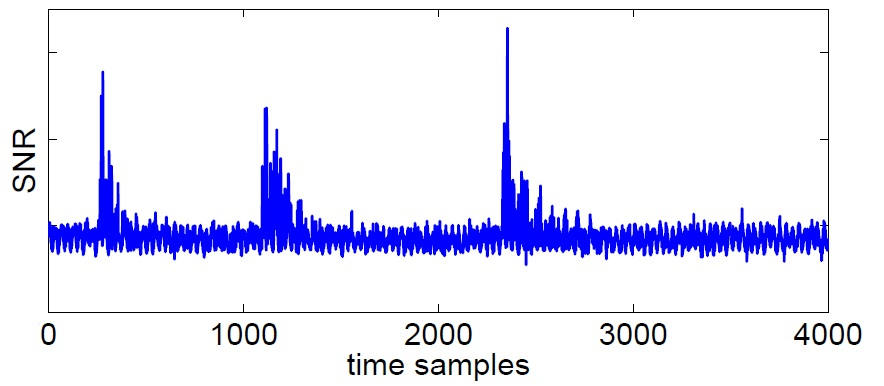
\includegraphics[width = \textwidth]{figures/SNR_1order_new.jpg} 
%\caption{$SNR(t) = {\frac{\text{\emph{variance inter-class}}}{\text{\emph{variance intra-class}}}}$}
%\end{figure}
%\end{column}
%\pause
%\begin{column}{0.5\textwidth}
%\textbf{Feature extraction - LDA}
%\begin{figure}
%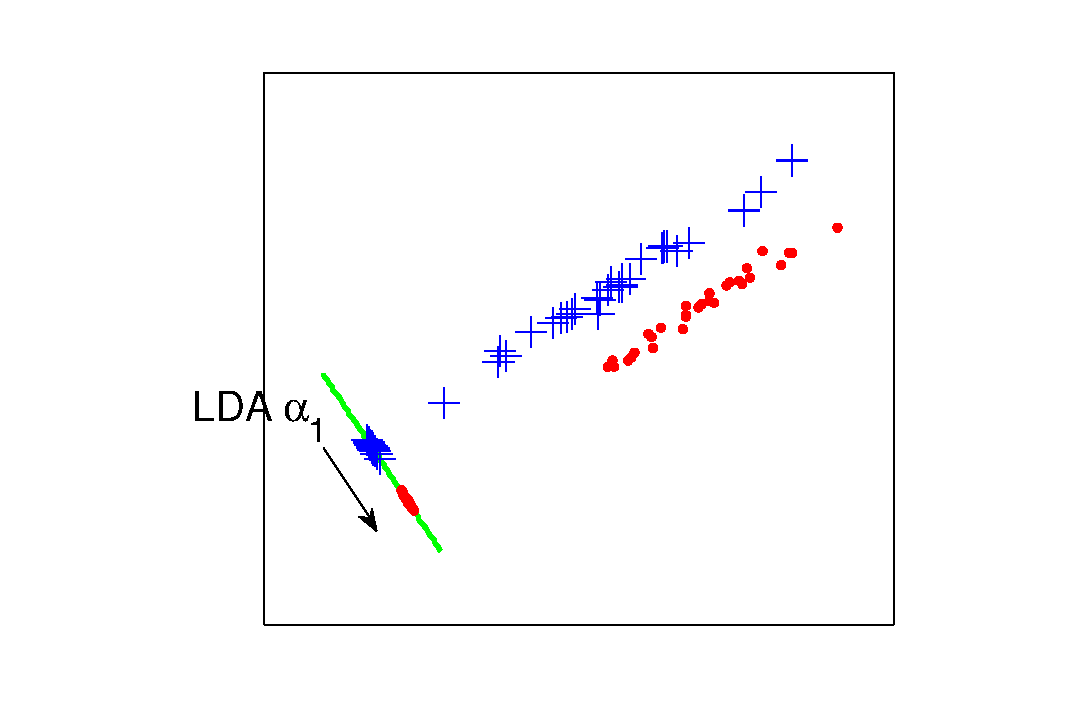
\includegraphics[width = 0.8\textwidth]{figures/LDAprojection.pdf} 
%\caption{Fisher's Criterion: project into a subspace in which  $\frac{\text{\emph{inter-class covariance matrix}}}{\text{\emph{intra-class covariance matrix}}}$ is maximised}
%\end{figure}
%\end{column}
%\end{columns}
%\pause
%LDA: optimal \textbf{classifier} under following hypothesis
%\begin{itemize}
%\item Gaussian distributions with parameters $\mu_j, \Sigma_j$
%\item Homoscedasticity: $\Sigma_j=\Sigma$ for all $j$
%\end{itemize}
%
%\begin{center}
%Fisher's criterion $\Leftrightarrow$ LDA 
%\end{center}
%\pause
%SNR and LDA most suitable selector and extractor for classification purposes
%
%\end{frame}


\begin{frame}

\frametitle{Contributions}

\begin{itemize}
\item \textbf{Linear Dimensionality Reduction} ([CARDIS 2015]): 
\begin{itemize}
\item PCA, choise of components ELV
\item LDA in case of undersampling
\end{itemize}

\item \only<1>{\textbf{Kernel Discriminant Analysis} ([CARDIS 2016]): application of an appropriate kernel trick to LDA, in order to manage masking countermeasure}\only<2->{\textcolor{red}{\textbf{Kernel Discriminant Analysis} ([CARDIS 2016]): application of an appropriate kernel trick to LDA, in order to manage masking countermeasure}}

\item \only<1>{\textbf{Convolutional Neural Networks} ([CHES 2017]):}\only<2->{\textcolor{red}{\textbf{Convolutional Neural Networks} ([CHES 2017]):}}
\begin{itemize}
\item \only<1>{discriminative model by means of neural network classifiers}\only<2->{\textcolor{red}{discriminative model by means of neural network classifiers}}
\item \only<1>{convolutional layers to manage desyncrhonisation (a form of hiding)}\only<2->{\textcolor{red}{convolutional layers to manage desyncrhonisation (a form of hiding)}}
\item \only<1>{Data Augmentation techniques to reduce overfitting}\only<2->{\textcolor{red}{Data Augmentation techniques to reduce overfitting}}
\end{itemize}

\item \textbf{ASCAD public dataset} (submitted paper):
\begin{itemize}
\item deep learning open comparison platform (implementation sources, side-channel traces, attack scripts)
\item hyper-parametrization methodology proposal and test
\end{itemize}
\end{itemize}


\end{frame}






%\begin{frame}
%\frametitle{Template Attack} 
%% aprendo des volets per ogni passaggio con riferimenti allo stato dell'arte:
%% templates : likelihood vs MAP ,  cov mats vs pooled , linear regression or not
%% dimensionality reduction : feature selection, feature extraction, masking : masques connus vs unconnus
%% misalignment : re-alignement
%
%\begin{tikzpicture}[ ->, node distance = 3cm,
%					decoration = {snake,   % <-- added
%                    pre length=3pt,post length=7pt,% <-- for better looking of arrow,
%                    }]
%
%\node [data] (db_profiling){
\includegraphics[width = 0.3\textwidth]{figures/database.jpg}\\ Profiling traces};
%\node [data, right of = db_profiling] (db_profiling_realigned){
\includegraphics[width = 0.3\textwidth]{figures/database.jpg}\\ \footnotesize{Realigned profiling traces}};
%\draw[arrow] (db_profiling) -- node[above]{$\rho$} (db_profiling_realigned) ;
%\node[function, above of = db_profiling, yshift=-1cm](realignment){$\rho$};
%\draw[arrow,dashed](db_profiling) -- (realignment);
%\node[function, above of= db_profiling_realigned, yshift=-1cm](extractor){$\varepsilon$};
%\node [data, right of = db_profiling_realigned] (extracted){
\includegraphics[width = 0.3\textwidth]{figures/database.jpg}\\ Profiling traces' features};
%\draw[arrow] (db_profiling_realigned) -- node[above]{$\varepsilon$} (extracted) ;
%\draw[arrow,dashed](db_profiling_realigned) -- (extractor);
%\node[data, right of = extracted, xshift=0.8cm](distributions){\small{$\mathrm{Pr}(\vaLeakVec \mid Z)$}\\
%\small{$\mathrm{Pr}(Z \mid \vaLeakVec)$}};
%\draw[arrow,dashed](extracted) -- node[above]{characterisation} (distributions);
%
%\node[methods, below of= db_profiling, yshift=1cm](realignments){Realignment \cite{nagashima2007dpa,van2011improving,durvaux2012efficient}};
%\node[methods, below of= db_profiling_realigned, yshift=1cm](extraction_methods){Dimensionality reduction};
%\node[methods, below of= extracted, yshift=1cm, align=left](charac_methods){\tiny{
%Template Attack \cite{Chari2003} (generative model, Gaussian hypothesis)\\
%\emph{Pooled} variant \cite{choudary2014efficient}\\
%Stochastic variant \cite{schindler2005stochastic}\\
%Discriminative model
%}};
%\node [data, below of=realignments, yshift=1cm ] (db_attack){
\includegraphics[width = 0.3\textwidth]{figures/database.jpg}\\ Attack traces};
%\node [data, right of = db_attack] (db_attack_realigned){
\includegraphics[width = 0.3\textwidth]{figures/database.jpg}\\ Realigned attack traces};
%\draw[arrow] (db_attack) -- node[above]{$\rho$} (db_attack_realigned) ;
%\node [data, right of = db_attack_realigned] (extracted_attack){
\includegraphics[width = 0.3\textwidth]{figures/database.jpg}\\ Attack traces' features};
%\draw[arrow] (db_attack_realigned) -- node[above]{$\varepsilon$} (extracted_attack) ;
%\node[data, right of = extracted_attack](keys){\footnotesize{$\mathrm{Pr}(K \mid \{ \vaLeakVec_i, P_i \}_{i=1,\dots,N})$}};
%\draw[arrow,dashed](extracted_attack) -- node[above]{inference} (keys);
%
%
%
%\end{tikzpicture}
%\end{frame}
%
%\begin{frame}
%\frametitle{Template Attack} 
%%% aprendo des volets per ogni passaggio con riferimenti allo stato dell'arte:
%%% templates : likelihood vs MAP ,  cov mats vs pooled , linear regression or not
%%% dimensionality reduction : feature selection, feature extraction, masking : masques connus vs unconnus
%%% misalignment : re-alignement
%%
%\begin{tikzpicture}[ ->, node distance = 2.5cm,
%				decoration = {snake,   % <-- added
%                   pre length=3pt,post length=7pt,% <-- for better looking of arrow,
%                   }]
%\uncover<4->{
%\node [data] (db_profiling){
\includegraphics[width = 0.3\textwidth]{figures/database.jpg}\\ Profiling traces};
%\node [data, right of = db_profiling] (db_profiling_realigned){
\includegraphics[width = 0.3\textwidth]{figures/database.jpg}\\ \footnotesize{Realigned profiling traces}};
%\draw[arrow] (db_profiling) -- node[above]{$\rho$} (db_profiling_realigned) ;
%\node[function, above of = db_profiling, yshift=-1cm](realignment){$\rho$};
%\draw[arrow,dashed](db_profiling) -- (realignment);
%\node[function, above of= db_profiling_realigned, yshift=-1cm](extractor){$\varepsilon$};
%\draw[arrow] (db_profiling_realigned) -- node[above]{$\varepsilon$} (extracted) ;
%\draw[arrow,dashed](db_profiling_realigned) -- (extractor);
%}
%
%\node [data, right of = db_profiling_realigned] (extracted){
\includegraphics[width = 0.3\textwidth]{figures/database.jpg}\\ \only<1>{Profiling traces} \only<3->{Profiling traces's features}};
%\node[data, right of = extracted, xshift=0.8cm](distributions){\small{$\mathrm{Pr}(\vaLeakVec \mid Z)$}};
%\draw[arrow,dashed](extracted) -- node[above]{characterisation} (distributions);
%
%\node[methods, below of= db_profiling, yshift=1cm](realignments){Realignment \cite{nagashima2007dpa,van2011improving,durvaux2012efficient}};
%\node[methods, below of= db_profiling_realigned, yshift=1cm](extraction_methods){Dimensionality reduction};
%\node[methods, below of= extracted, yshift=1cm, align=left](charac_methods){\tiny{
%Template Attack \cite{Chari2003} (generative model)\\
%\uncover<3->{\emph{Pooled} variant \cite{choudary2014efficient}\\
%Stochastic variant \cite{schindler2005stochastic}}
%}};
%
%\only<4->{
%\node [data, below of=realignments, yshift=1cm ] (db_attack){
\includegraphics[width = 0.3\textwidth]{figures/database.jpg}\\ Attack traces};
%\node [data, right of = db_attack] (db_attack_realigned){
\includegraphics[width = 0.3\textwidth]{figures/database.jpg}\\ Realigned attack traces};
%\draw[arrow] (db_attack) -- node[above]{$\rho$} (db_attack_realigned) ;
%}
%\node [data, right of = db_attack_realigned] (extracted_attack){
\includegraphics[width = 0.3\textwidth]{figures/database.jpg}\\ \only<1-2>{Attack traces} \only<3->{Attack traces' features}};
%\draw[arrow] (db_attack_realigned) -- node[above]{$\varepsilon$} (extracted_attack) ;
%\node[data, right of = extracted_attack](keys){Maximum Likelihood or Maximum A Posteriori};
%\draw[arrow,dashed](extracted_attack) -- node[above]{inference} (keys);
%
%
%
%\end{tikzpicture}
%\end{frame}
%